\documentclass{beamer}

\usetheme{Madrid}
\usepackage{amsmath, amssymb}
\usepackage{graphicx}
\usepackage{booktabs}

\newtheorem{assumption}{Assumption}

\title{Proximal Drift-Plus-Penalty}
\subtitle{Time-Varying Constraints: $h_t = h + \psi_t$}
\author{}
\date{\today}

\begin{document}

\begin{frame}
  \titlepage
\end{frame}

% ------------------------------------------------------------------
\begin{frame}{Overview}
  \small
  \textbf{Primal problem (time-varying):}
  \[
    \min_{x \in X} f(x) \quad \text{s.t.} \quad g(x) \le 0,
    \qquad \limsup_{T\to\infty} \tfrac1T \sum_{t=1}^T h_t(x_t) \le 0
  \]

  \textbf{Penalized objective:}
  \[
    P(x) = f(x) + \beta\,[g(x)]_+
  \]

  \textbf{Algorithm (per step $t$, $q_t := Q_t/V$, observing $h_t$):}
  \begin{align*}
    x_{t+1} &= \operatorname*{arg\,min}_{x \in X} P(x) + q_t\big(h_t(x)+\gamma\|x-x_t\|^2\big) + \tfrac{1}{2\eta}\|x-x_t\|^2 \\
    Q_{t+1} &= \max(Q_t + h_t(x_{t+1}),\,0)
  \end{align*}
\end{frame}

% ------------------------------------------------------------------
\begin{frame}{Domain and Function Definitions}
  \[
    X = \{\, x \in \mathbb{R}^d : \|x\| \le R_X \,\} \qquad D := \operatorname{diam}(X) = 2R_X
  \]

  \[
    f(x) = \tfrac{1}{2} w^f_{\mathrm{quad}}\|x\|^2 \;-\; c_f^\top x \;+\; \sum_{j=1}^{6} \alpha^f_j \cos\big(w^f_j \cdot x + b^f_j\big)
  \]

  \[
    g(x) = \|x\|^2 - r_g^2
  \]

  \[
    h_t(x) = \underbrace{\tfrac{1}{2} w^h_{\mathrm{quad}}\|x\|^2 \;+\; \sum_{j=1}^{3} \alpha^h_j \cos\big(w^h_j \cdot x + b^h_j\big) \;+\; \text{offset}_h}_{h(x),\ \text{fixed}} \;+\; \underbrace{\psi_t}_{\text{drifts each round}}
  \]

  \begin{itemize}
    \item $g$: exactly convex ball: kept this way so $\kappa_g = 2\beta r_g$ (Assumption 6) holds
    \item $\psi_t$: additive scalar drift, constant in $x$: does not change $h$'s shape, only its offset
  \end{itemize}
\end{frame}

% ------------------------------------------------------------------
\begin{frame}{Synthetic Instance: Exact Parameters}
  \small
  $d=10$, \ $R_X=1$, \ $r_g=0.75$, \ $\xi=0.4$, \ $D=2$, \ seed $=0$

  \vspace{0.3em}
  $w^f_{\mathrm{quad}}=0.2$, \ $\|c_f\|=0.5$ \quad\quad $w^h_{\mathrm{quad}}=2.0$, \ offset$_h=-0.400722$

  \vspace{0.5em}
  \centering
  \begin{tabular}{c|rrrrrr}
    \multicolumn{7}{c}{$f$: 6 cosine terms} \\
    \hline
    $j$ & 1 & 2 & 3 & 4 & 5 & 6 \\
    $\alpha^f_j$ & 0.20 & 0.20 & 0.20 & 0.20 & 0.20 & 0.20 \\
    $\|w^f_j\|$ & 1.00 & 1.24 & 1.48 & 1.72 & 1.96 & 2.20 \\
    $b^f_j$ & 4.00 & 1.70 & 0.26 & 0.10 & 5.11 & 5.74 \\
  \end{tabular}

  \vspace{0.6em}
  \begin{tabular}{c|rrr}
    \multicolumn{4}{c}{$h$: 3 cosine terms} \\
    \hline
    $j$ & 1 & 2 & 3 \\
    $\alpha^h_j$ & 0.025 & 0.025 & 0.025 \\
    $\|w^h_j\|$ & 1.00 & 1.25 & 1.50 \\
    $b^h_j$ & 5.96 & 2.89 & 4.76 \\
  \end{tabular}

  \vspace{0.6em}
  \footnotesize (direction vectors $w^f_j/\|w^f_j\|$, $w^h_j/\|w^h_j\|$, and $c_f/\|c_f\|$: random unit vectors, seed$=0$ -- omitted here, 10 components each)

  \vspace{0.6em}
  \normalsize
  $\Rightarrow\ \rho_f = 3.274$, \ $\rho_h = 0.120$, \ $L_f = 2.620$, \ $L_h = 2.094$, \ $H = 1.476$, \ $G_g = 0.438$
\end{frame}

% ------------------------------------------------------------------
\begin{frame}{Hyperparameters}
  \small
  \textbf{Algorithm:}
  \begin{center}
  \begin{tabular}{cccccc}
    \toprule
    $\beta$ & $\gamma$ & $\eta$ & $V$ & $T$ \\
    \midrule
    679.0 & 0.065 & 0.2 & 20.0 & 4000 \\
    \bottomrule
  \end{tabular}
  \end{center}

  \vspace{0.5em}
  \textbf{Derived windows (must contain the chosen $\gamma,\eta$):}
  \[
    \gamma \in \left(\tfrac{\rho_h}{2},\ \tfrac{\xi}{D^2}\right) = (0.060,\ 0.100)
    \qquad\qquad
    \eta \in \left(0,\ \tfrac{1}{\rho_f}\right) = (0,\ 0.305)
  \]

  \vspace{0.5em}
  \textbf{Drift $\psi_t$:}
  \begin{center}
  \begin{tabular}{ccc}
    \toprule
    $\psi_{\max}$ (valid) & $\psi_{\max}$ (Slater-violating) & drift seed \\
    \midrule
    0.08 & 0.6 & 11 \\
    \bottomrule
  \end{tabular}
  \end{center}

  \vspace{0.5em}
  \textbf{Sweep grids:}
  \begin{itemize}
    \item $V \in \{0.1, 0.25, 0.5, 1, 2, 5, 10, 20, 50, 100\}$
    \item $\beta \in \{0.01, 0.05, 0.1, 0.2, 0.3, 0.4, 0.5, 1, 5, 20, 50, 100, 300, 679, 800\}$
  \end{itemize}
\end{frame}

% ------------------------------------------------------------------
\begin{frame}{The Drift Mechanism}
  \small
  $\psi_t$ is generated \emph{once}, before the run starts -- the algorithm only ever sees $\psi_t$ at round $t$, never the future.

  \vspace{0.5em}
  \textbf{Slow drift} (small upward bias + noise, clipped):
  \[
    \psi_{t+1} = \operatorname{clip}\big(\psi_t + 0.0006 + \mathcal N(0, 0.012^2),\ 0,\ \psi_{\max}\big)
  \]

  \textbf{Bursts} (mostly flat, occasional jumps that decay back down):
  \[
    \text{level}_{t+1} = 0.997 \cdot \text{level}_t \;+\; \mathbb 1[\text{burst at } t]\cdot \psi_{\max}\cdot\text{Unif}(0.5,1.0)
  \]
  \[
    \psi_t = \operatorname{clip}\big(\text{level}_t + \mathcal N(0, 0.004^2),\ 0,\ \psi_{\max}\big)
  \]

  \vspace{0.5em}
  \textbf{Functional variation} (what the theory's $V_T$ term measures):
  \[
    \Delta_t = |\psi_{t+1}-\psi_t| \qquad\qquad V_T = \sum_{t=1}^{T-1}\Delta_t
  \]

  \begin{block}{Why $\psi_t$ alone determines $\Delta_t$}
    \small $h_{t+1}(x)-h_t(x) = \psi_{t+1}-\psi_t$ for \emph{every} $x$ -- the $h(x)$ part cancels exactly, so the functional variation reduces to a 1-D quantity.
  \end{block}
\end{frame}

% ==================================================================
% RESULTS
% ==================================================================

% ------------------------------------------------------------------
\begin{frame}{One Trajectory (Burst Drift)}
  \centering
  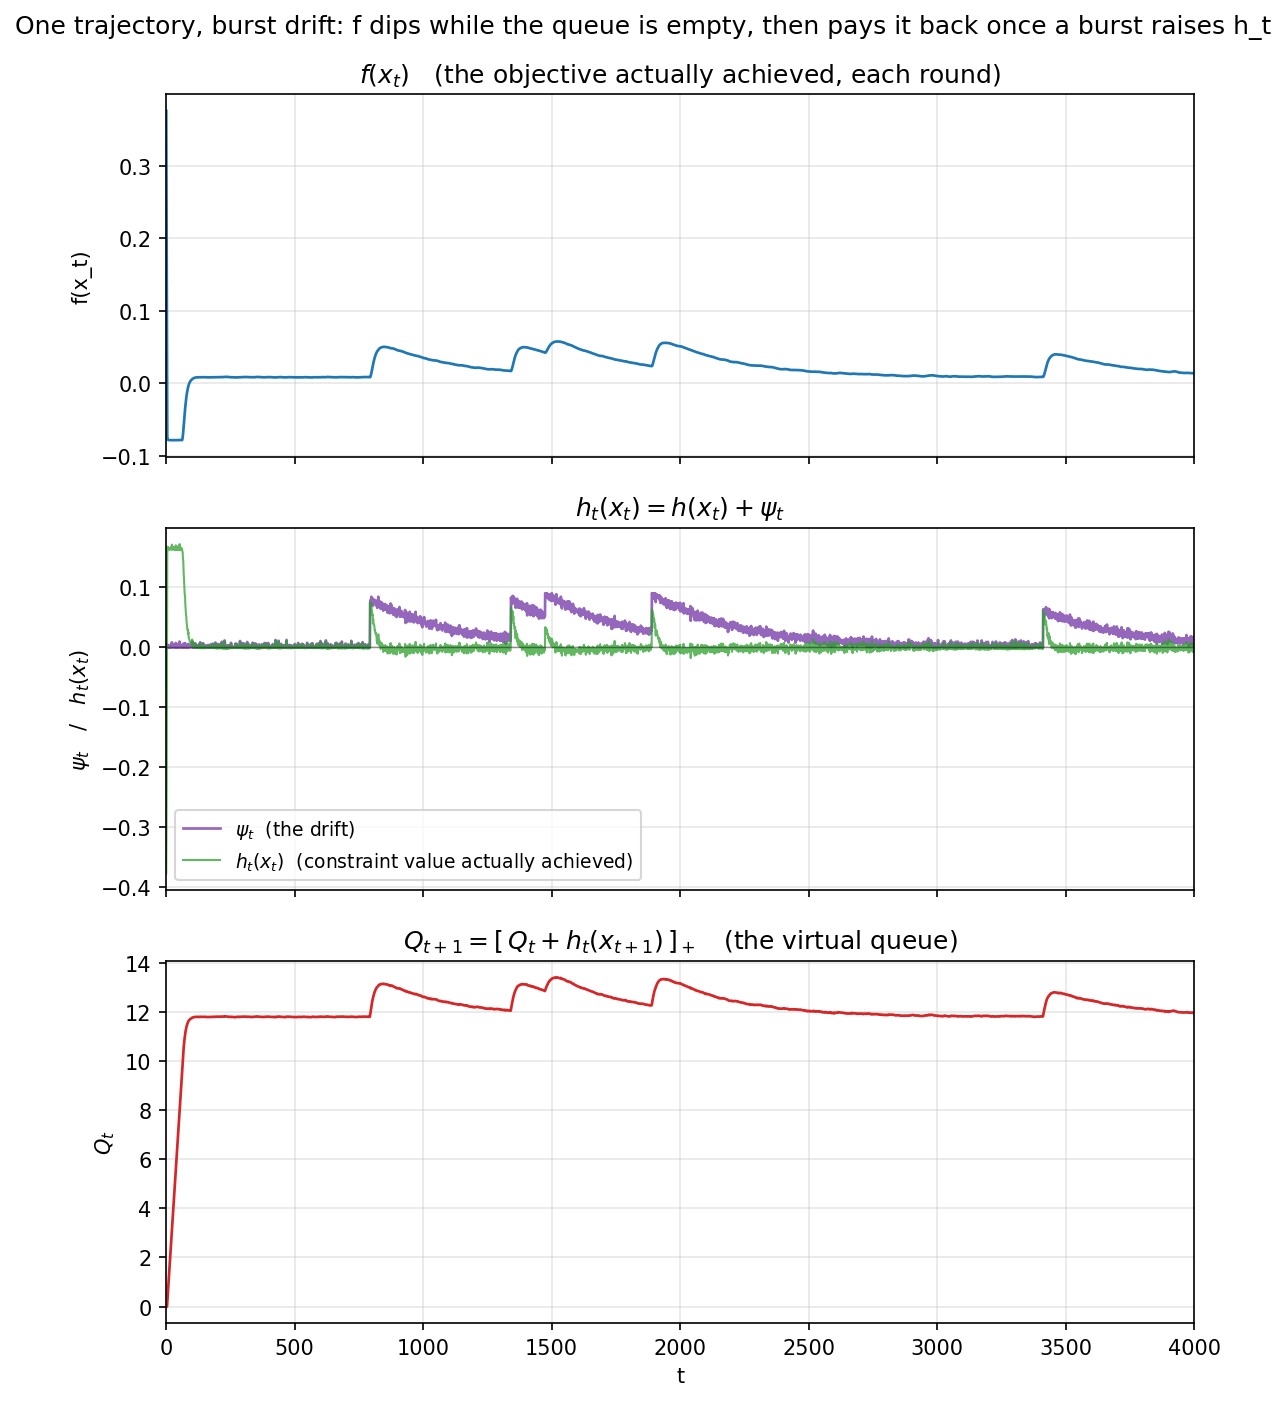
\includegraphics[height=0.82\textheight]{../figures/time_varying/trajectory_tv.png}
\end{frame}

% ------------------------------------------------------------------
\begin{frame}{Lemma 2: Pointwise Queue Bound}
  \centering
  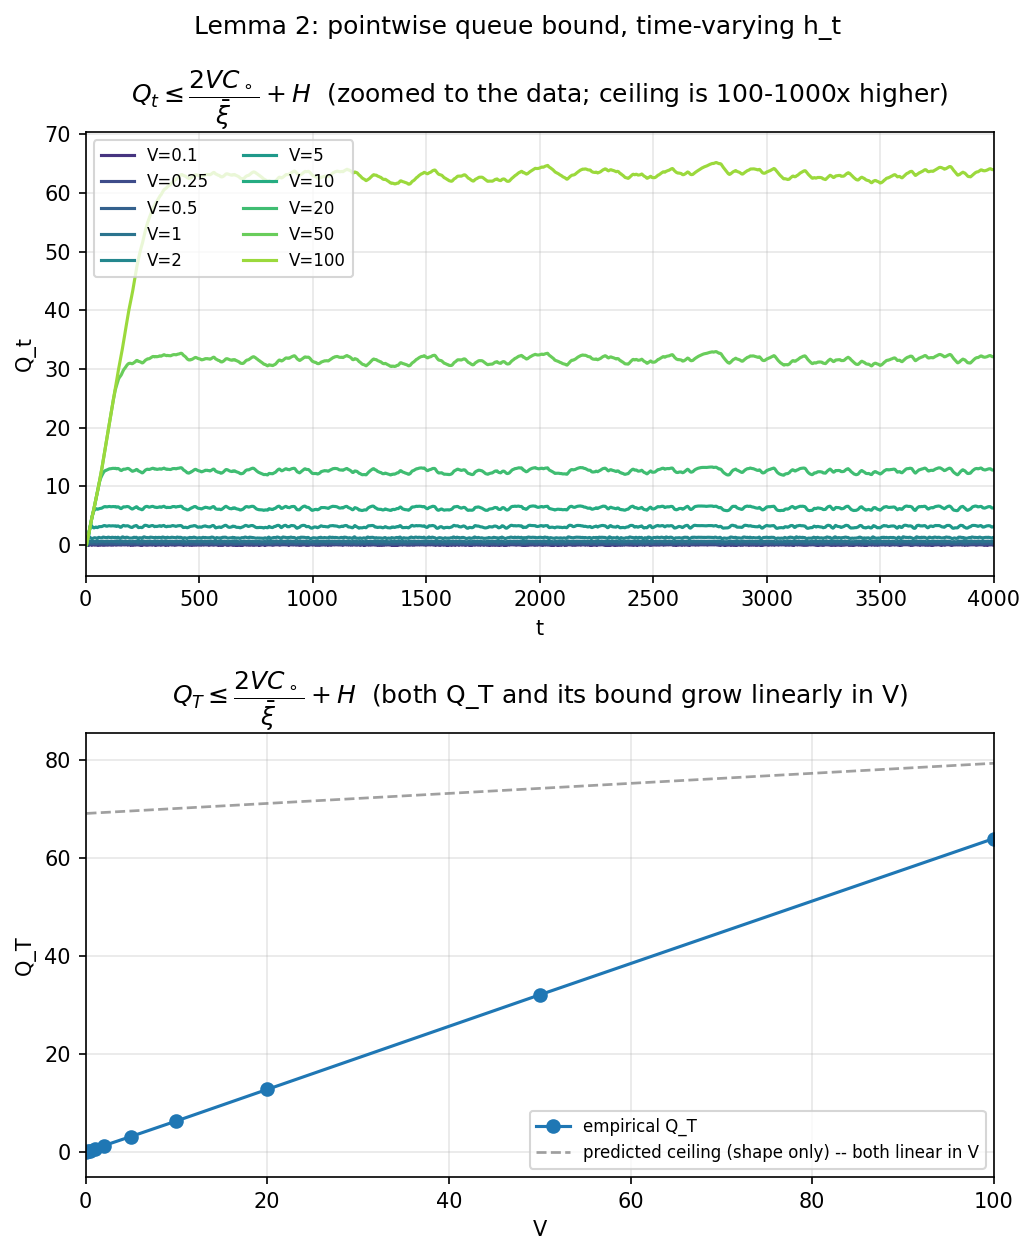
\includegraphics[height=0.82\textheight]{../figures/time_varying/lemma2_queue_tv.png}
\end{frame}

% ------------------------------------------------------------------
\begin{frame}{Definition 1: One-Step Functional Variation}
  \centering
  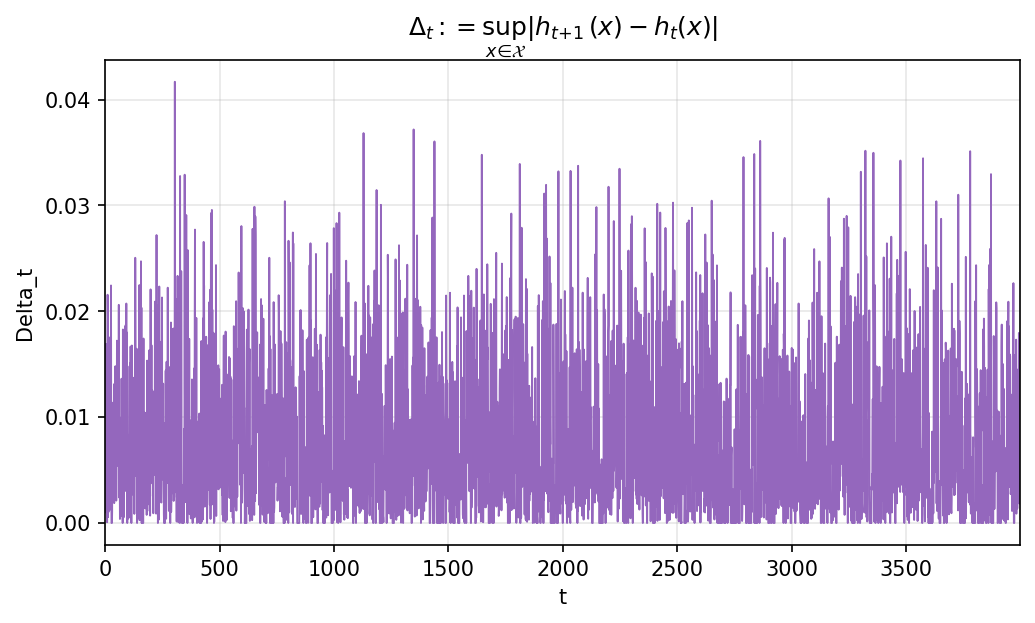
\includegraphics[width=0.75\textwidth]{../figures/time_varying/delta_t_variation.png}
\end{frame}

% ------------------------------------------------------------------
\begin{frame}{Definition 1: Cumulative Functional Variation}
  \centering
  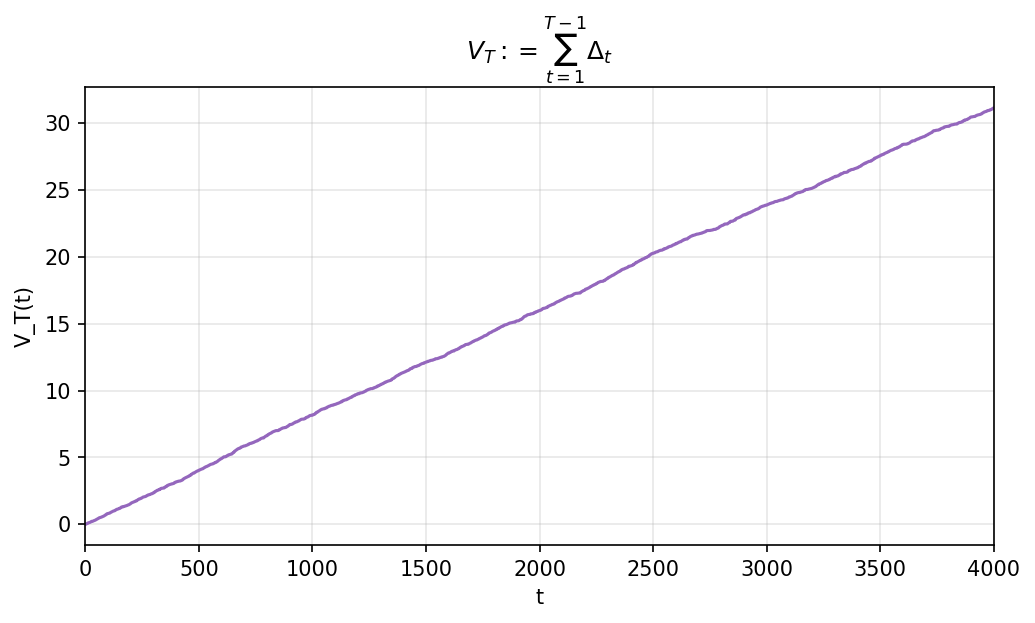
\includegraphics[width=0.75\textwidth]{../figures/time_varying/cumulative_VT_tv.png}
\end{frame}

% ------------------------------------------------------------------
\begin{frame}{Theorem 1: Time-Average Feasibility, vs $t$}
  \centering
  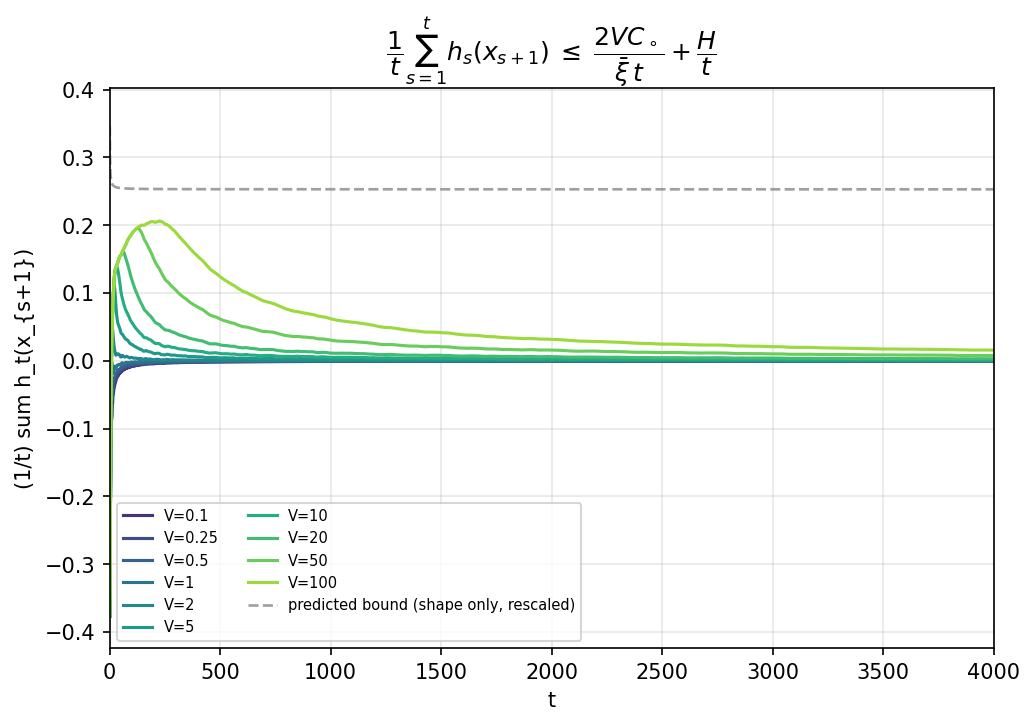
\includegraphics[width=0.72\textwidth]{../figures/time_varying/theorem1_vs_t.png}
\end{frame}

% ------------------------------------------------------------------
\begin{frame}{Theorem 1: Time-Average Feasibility, vs $V$}
  \centering
  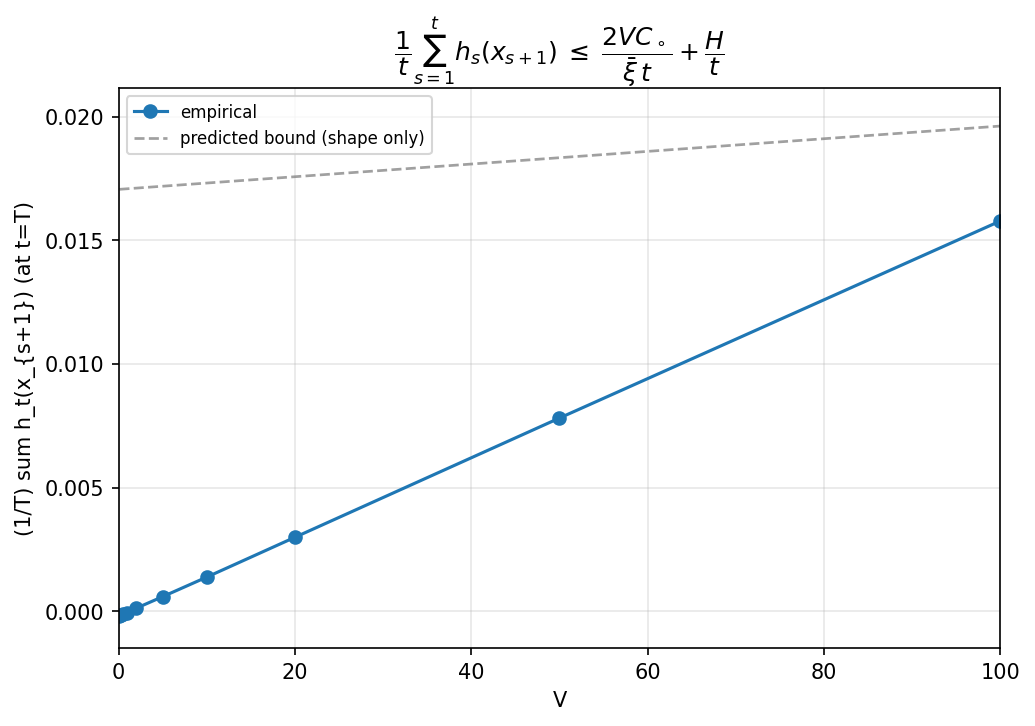
\includegraphics[width=0.72\textwidth]{../figures/time_varying/theorem1_vs_V.png}
\end{frame}

% ------------------------------------------------------------------
\begin{frame}{Theorem 2 (Movement), vs $t$}
  \centering
  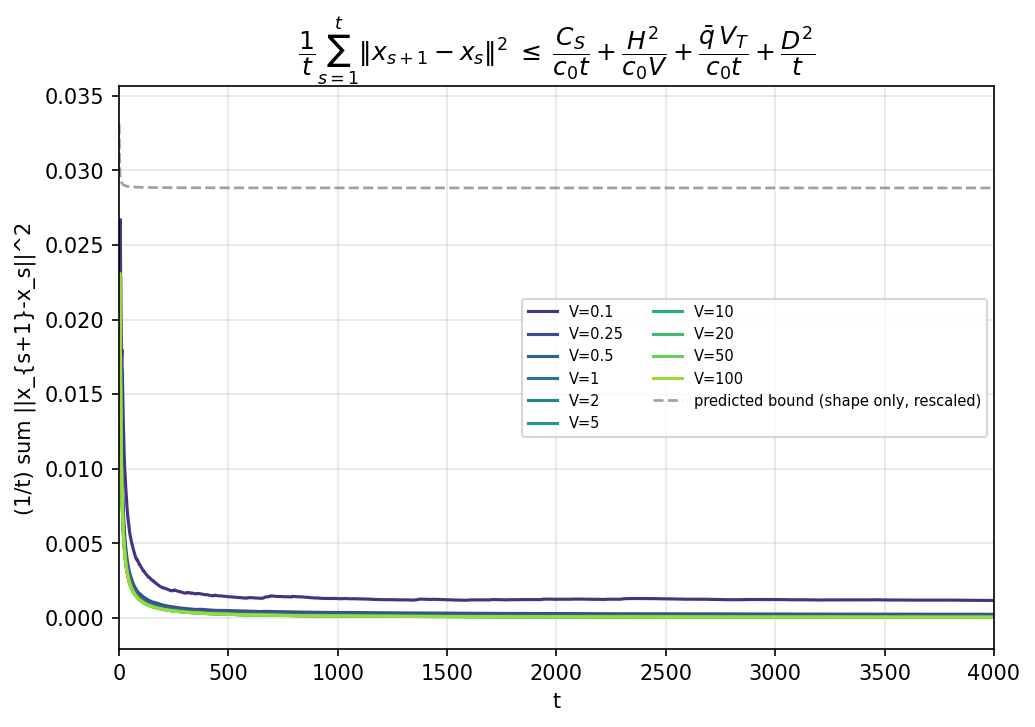
\includegraphics[width=0.72\textwidth]{../figures/time_varying/theorem2_movement_vs_t.png}
\end{frame}

% ------------------------------------------------------------------
\begin{frame}{Theorem 2 (Movement), vs $V$}
  \centering
  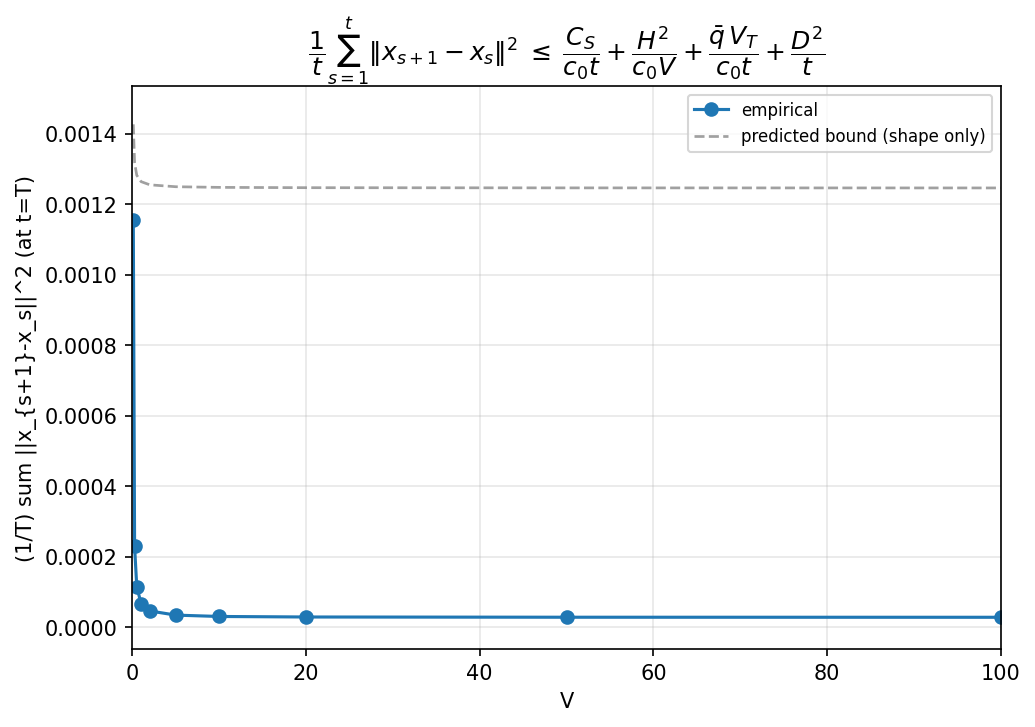
\includegraphics[width=0.72\textwidth]{../figures/time_varying/theorem2_movement_vs_V.png}
\end{frame}

% ------------------------------------------------------------------
\begin{frame}{Theorem 2 (Near-Stationarity Residual), vs $t$}
  \centering
  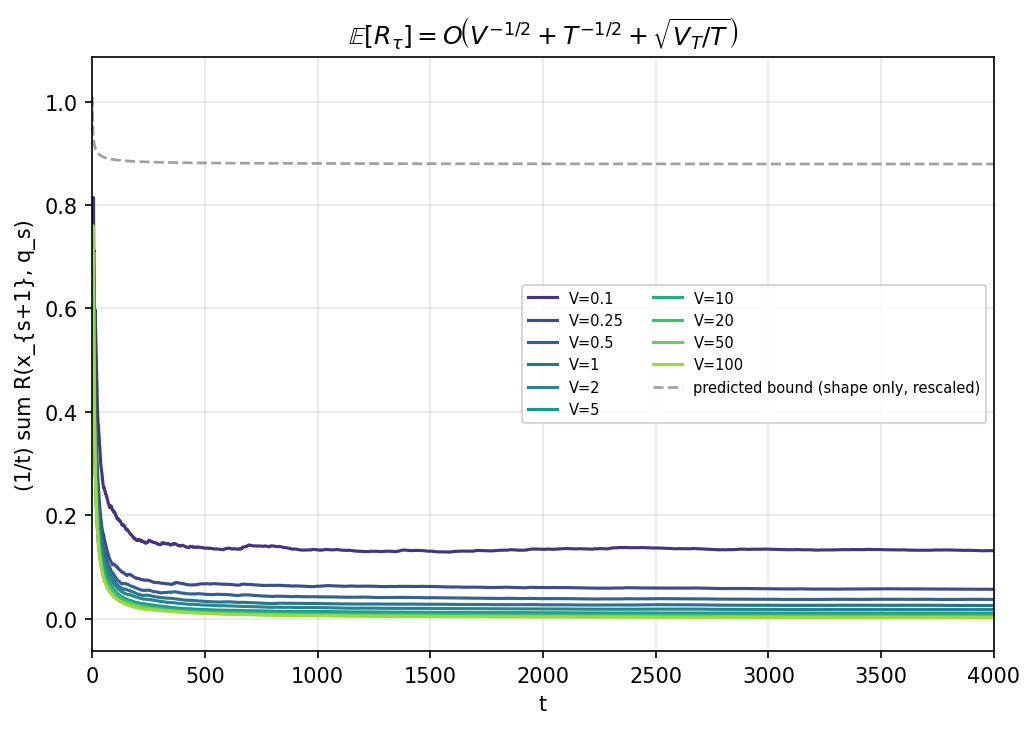
\includegraphics[width=0.72\textwidth]{../figures/time_varying/theorem2_residual_vs_t.png}
\end{frame}

% ------------------------------------------------------------------
\begin{frame}{Theorem 2 (Near-Stationarity Residual), vs $V$}
  \centering
  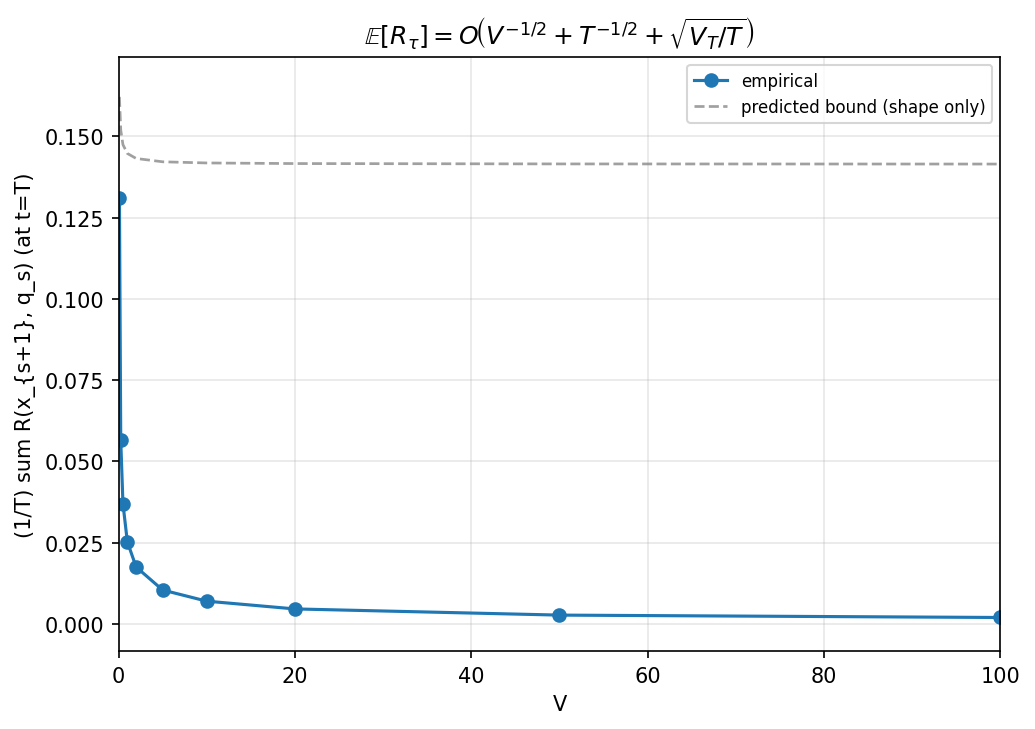
\includegraphics[width=0.72\textwidth]{../figures/time_varying/theorem2_residual_vs_V.png}
\end{frame}

% ------------------------------------------------------------------
\begin{frame}{Theorem 3 (Nearly-feasible stationarity for the ordinary constraint), vs $t$}
  \centering
  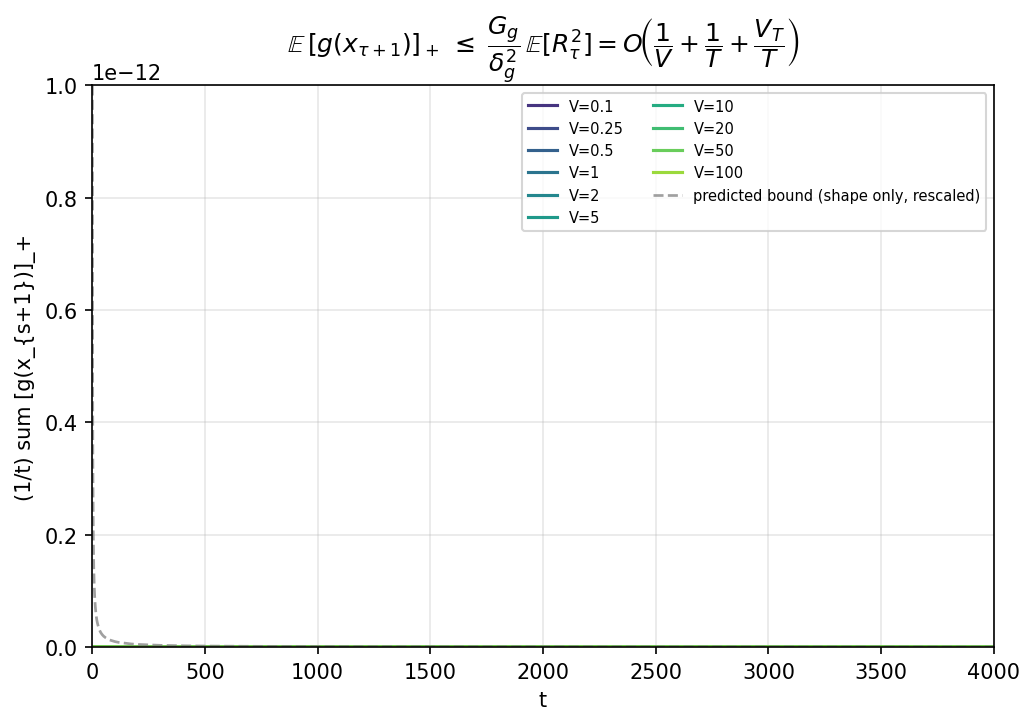
\includegraphics[width=0.72\textwidth]{../figures/time_varying/theorem3_valid_vs_t.png}
\end{frame}

% ------------------------------------------------------------------
\begin{frame}{Theorem 3 (Nearly-feasible stationarity for the ordinary constraint), vs $V$}
  \centering
  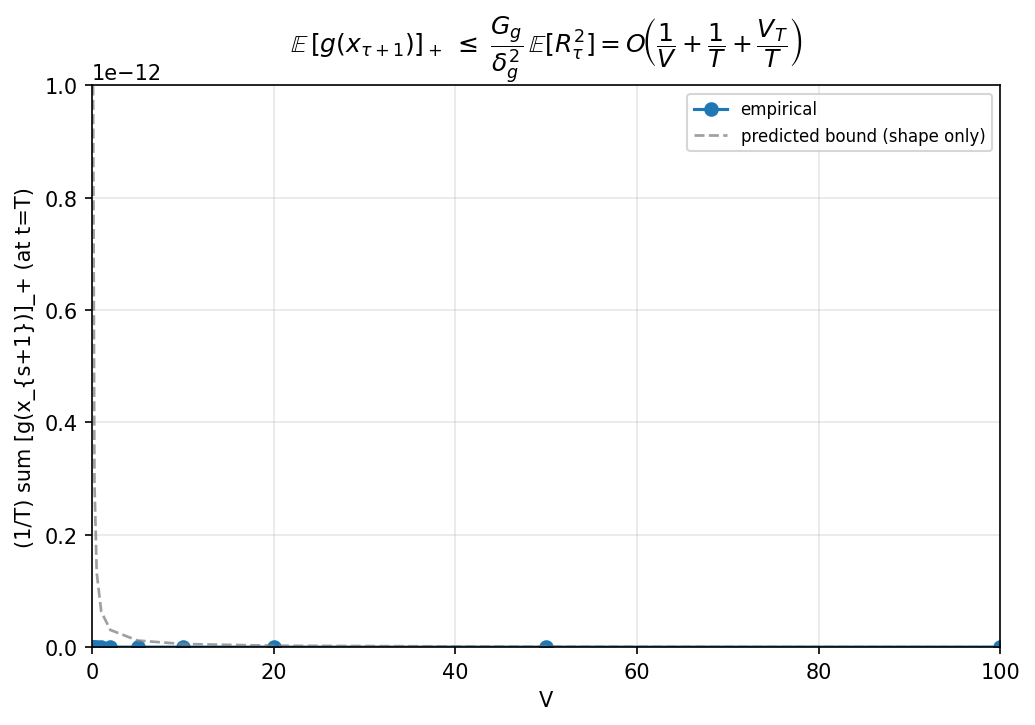
\includegraphics[width=0.72\textwidth]{../figures/time_varying/theorem3_valid_vs_V.png}
\end{frame}

% ------------------------------------------------------------------
\begin{frame}{Theorem 3 (Dangerous Instance, $\beta=0.4$), vs $t$}
  \centering
  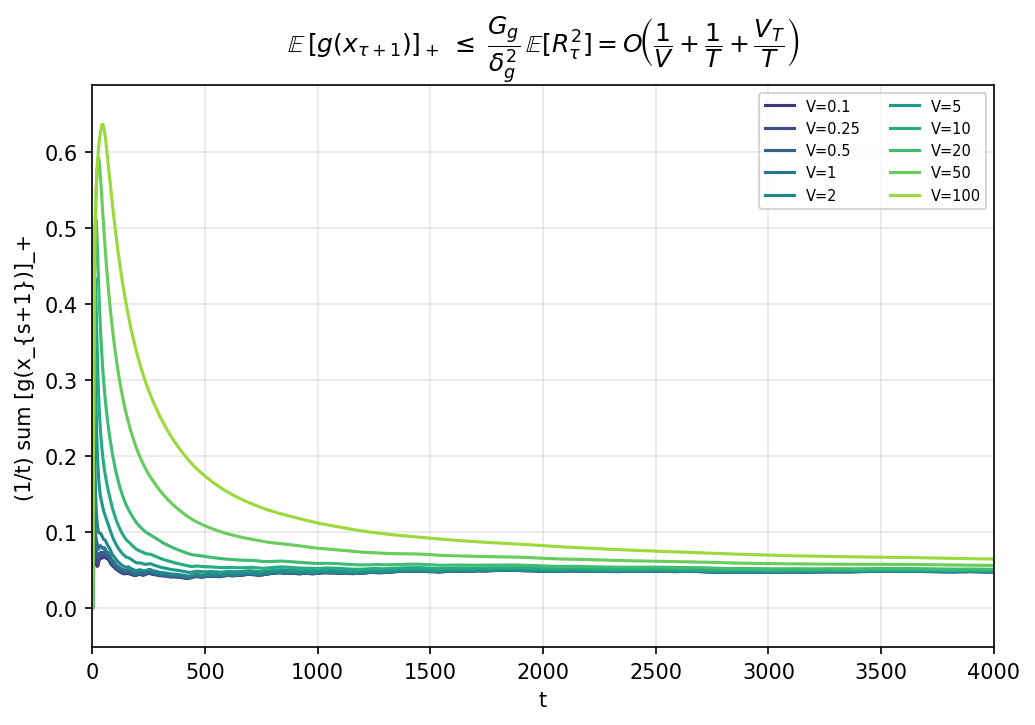
\includegraphics[width=0.72\textwidth]{../figures/time_varying/theorem3_vs_t.png}
\end{frame}

% ------------------------------------------------------------------
\begin{frame}{Theorem 3 (Dangerous Instance, $\beta=0.4$), vs $V$}
  \centering
  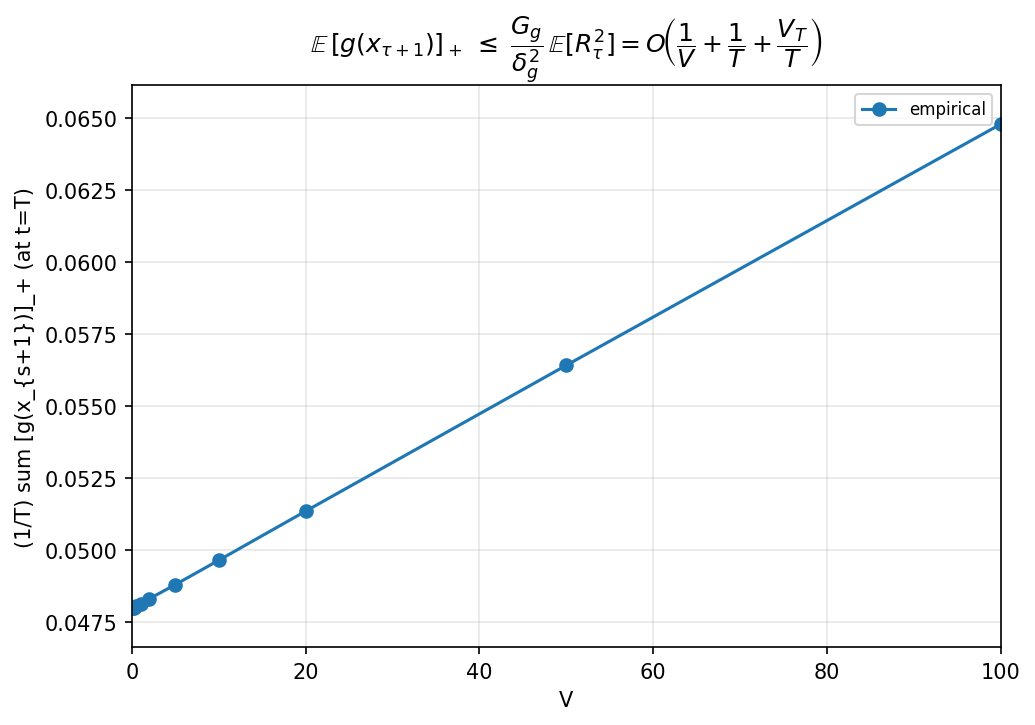
\includegraphics[width=0.72\textwidth]{../figures/time_varying/theorem3_vs_V.png}

  \footnotesize Bigger $V$ weakens the queue's restraint on $h_t$ (which also pulls inward here) while $\beta$'s restraint stays fixed -- so violation \emph{grows} with $V$, opposite the theorem's own $O(1/V)$ rate, which assumed $\delta_g>0$.
\end{frame}

% ------------------------------------------------------------------
\begin{frame}{Theorem 3: $\beta$ Sweep (Original Instance)}
  \centering
  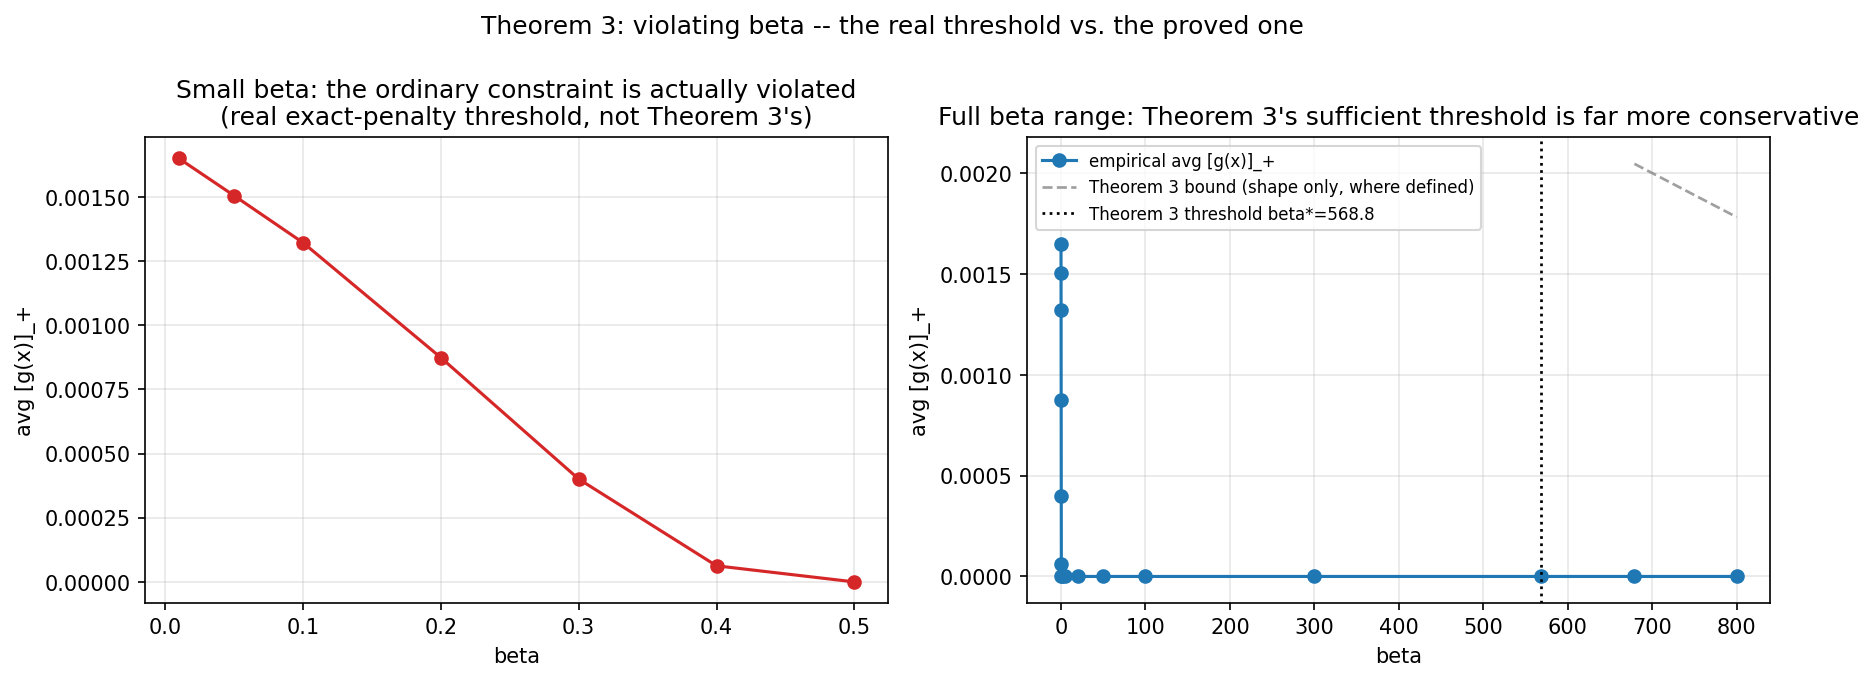
\includegraphics[width=0.95\textwidth]{../figures/time_varying/theorem3_beta_violation_tv.png}

  \footnotesize Real threshold ($\approx0.5$) vs. Theorem 3's own threshold ($\beta^\star\approx569$) -- about 1100$\times$ apart, from stacking a worst-case $\bar q$, Markov's inequality, and a worst-case regularity constant $\kappa_g$.
\end{frame}

\end{document}
